\chapter{Microsoft Teams lesson management - some examples}\label{appendices:ms_teams}

With the COVID-19 outbreak, \acrshort{fhict} switched activity form face-to-face to the online environment, \acrshort{msteams} becoming an essential tool to conduct education. Below are some examples of lesson management using \acrshort{msteams}.
Note that due to the \acrfull{gdpr} regulations, the examples show mock people.

\begin{figure}[h]
    \centering
    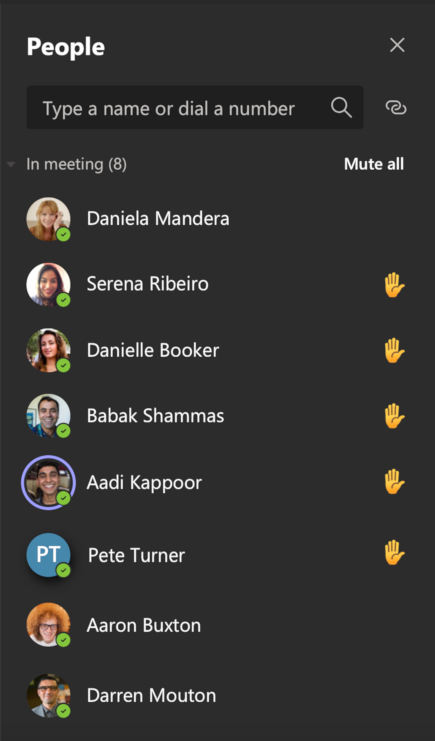
\includegraphics[width = 0.45\textwidth]{appendices/ms_teams/ms_teams_images/mircosoft_rise_your_hand.jpg}
    \caption{Microsoft Teams "Rise your hand" feature dealing with the visual impediment of virtual lessons when a question is raised (source: \url{https://support.content.office.net/en-us/media/2339be3c-e810-4ca1-aad3-f4536c8f0c4f.jpg})
    }
    \label{fig:my_label}
\end{figure}

\begin{figure}
    \centering
    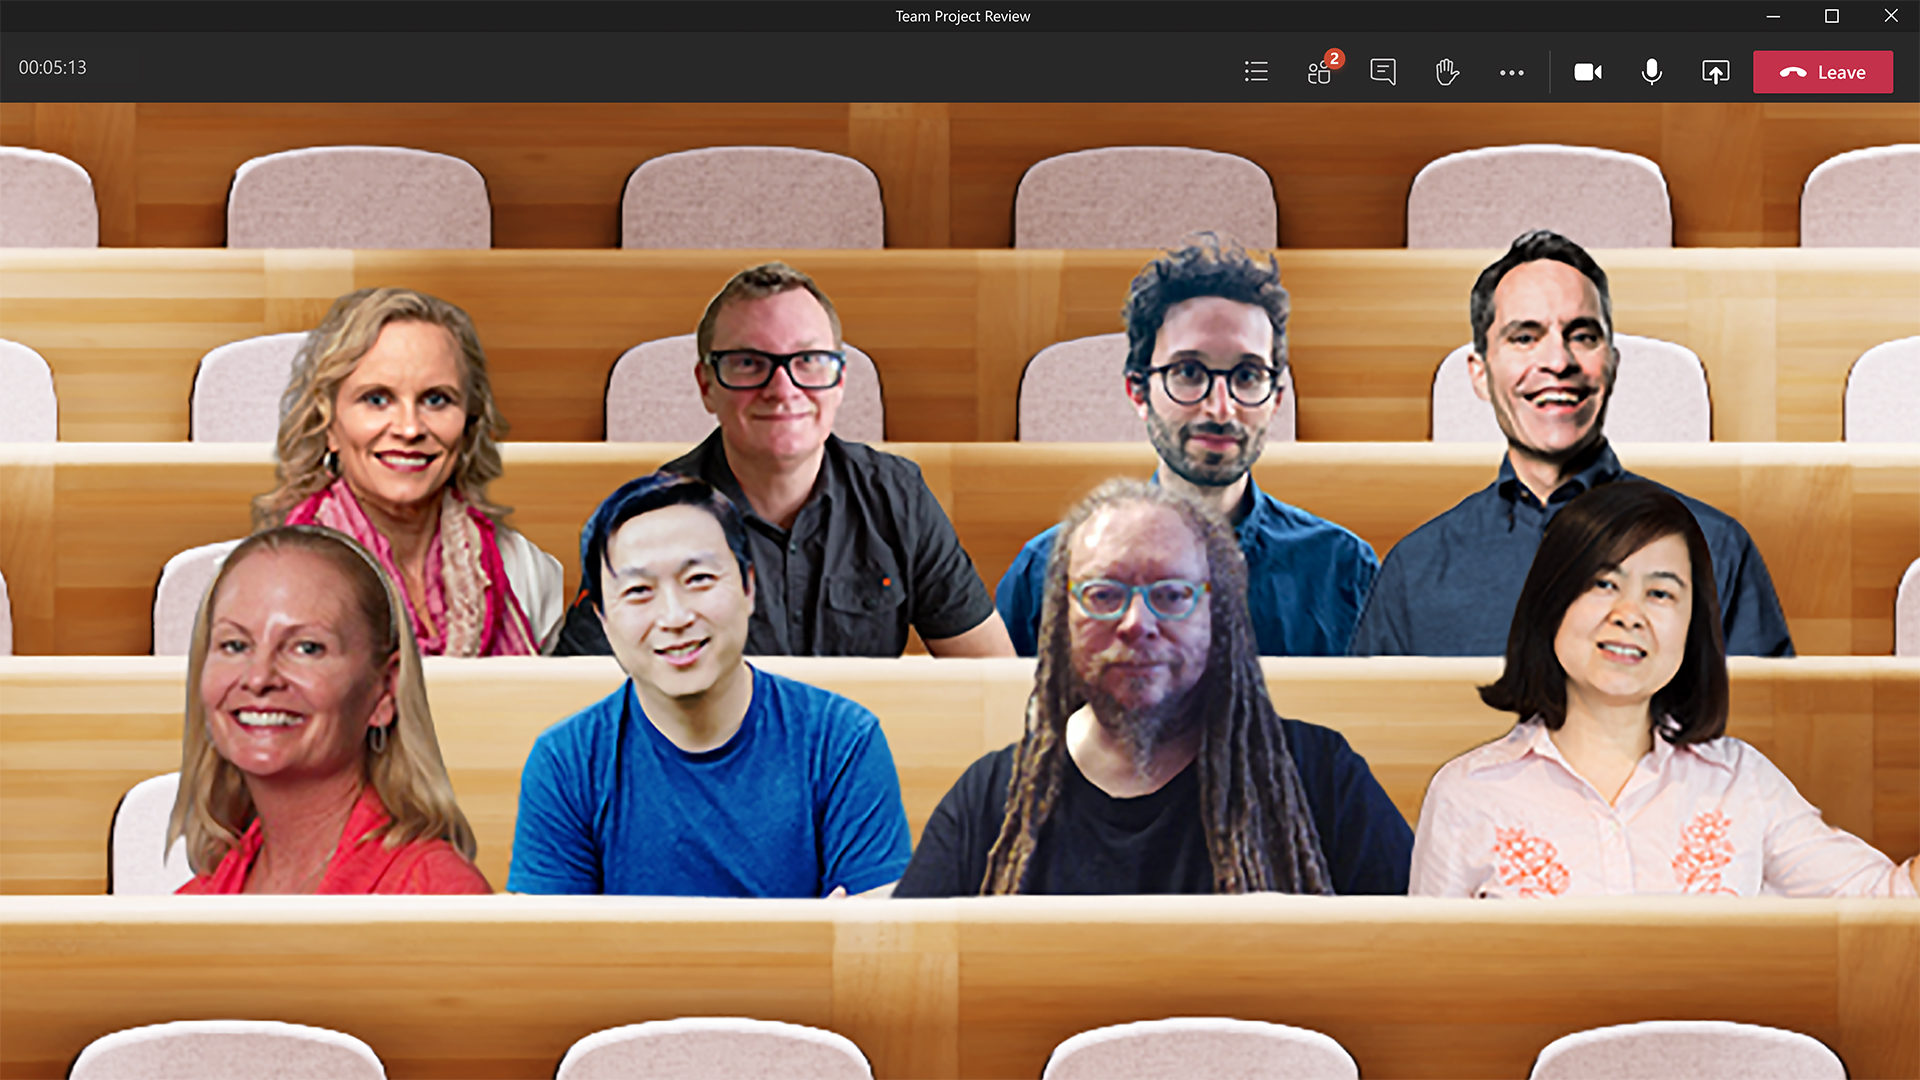
\includegraphics[width=\textwidth]{appendices/ms_teams/ms_teams_images/mircosoft_together_mode.jpg}
    \caption{Microsoft Teams "Together mode" feature (source: \url{https://news.microsoft.com/innovation-stories/microsoft-teams-together-mode/})}
    \label{fig:my_label}
\end{figure}

\begin{figure}[h]
    \centering
    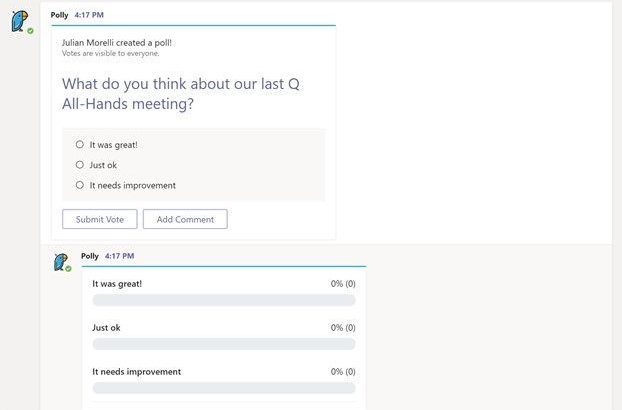
\includegraphics[width=\textwidth]{appendices/ms_teams/ms_teams_images/mircosoft_polly.jpg}
    \caption{Microsoft Teams Polly extension (source: \url{https://techcommunity.microsoft.com/t5/image/serverpage/image-id/54572i5530143C4F2B7577/image-size/large?v=1.0&px=999})}
    \label{fig:my_label}
\end{figure}
